\section{Evaluation}
Da nun der ganze Funktionsumfang inklusive Wireframes, Objekten und deren
Objektattributen bekannt ist, können die möglichen Technologien und Tools
gewählt werden.

Hierzu stellt sich die Frage, welche Technologien und Tools stehen überhaupt
zur Verfügung, um einen solchen Prototypen umzusetzen und was für Kriterien spielen
dazu eine Rolle.

In der Tabelle \ref{tab:umsetzungskriterien} liste ich die Kriterien auf, die
meiner Meinung nach einen Einfluss auf die Wahl haben und stelle eine klaren 
Frage, die ich in einem weiteren Schritt beantworten und erläutern werde.

\begin{table}[h]
\begin{center}
    \begin{tabular}{llp{9cm}l}
        \toprule Nr & Kriterium & Beschreibung \\
        \midrule 1 & Zielsystem & Damit ist die Plattform der Endbenutzer
                 gemeint. Auf welchen Betriebssystemen soll der Prototyp 
                 verwendet werden können? \\
        \midrule 2 & Programmiersprache & In welcher Programmiersprache soll
                 der Prototyp geschrieben werden? \\
        \midrule 3 & Framework & Welches Framework soll als Unterstützung zur
                 Programmiersprache verwendet werden? \\
        \midrule 4 & Versionsverwaltungssystem & Welches Versionsverwaltungssystem soll
                 verwendet werden, um den öffentlichen Quellcode zu verwalten? \\
        \midrule 5 & Meine Kenntnisse & Über welche Kenntnisse verfüge ich, um
                 den Prototypen in einer angemessenen Zeit umzusetzen? \\
        \bottomrule
    \end{tabular}
    \caption{Kriterien mit Einfluss auf die Wahl der Technologien und Tools}
    \label{tab:umsetzungskriterien}
\end{center}
\end{table}

Das letzte Kriterium Nr. 5 ``Meine Kenntnisse'' werde ich nicht einzeln abhandeln,
da es einen Einfluss auf alle anderen Kriterien hat und somit sowieso in die Wahl
einfliesst.

Grundsätzlich ist zu erwähnen, dass dieses Kriterium das am stärksten
gewichtete ist, da es den grössten Einfluss auf die Umsetzungszeit und die
Qualität hat. Ich habe jedoch während den letzten Jahren mehrere Webapplikationen
umgesetzt und habe somit nicht das Gefühl, dass dies einen schlechten Einfluss
auf meine Wahl haben wird. 
 
\subsection{Zielsystem}
Grundsätzlich möchte ich, dass der Prototyp von möglichst vielen Betriebssystemen
verwendet werden kann. Es gibt eine Vielzahl von Betriebssystemen \cite{betriebssysteme}
und das Internet bietet hierzu eine gute Möglichkeit betriebssystemübergreiffende
Applikationen zu erstellen. Hinzu kommt, dass alle bestehenden Plattformen,
die ich untersucht habe, als Webapplikation implementiert sind. Deshalb denke ich, 
dass das auch die richtige Wahl für meinen Prototypen ist.

\subsection{Programmiersprache}
Auch hier gibt es fast unzählige mögliche Programmiersprachen. Durch die Wahl
einer Webapplikation können diese noch mehr eingeschränkt werden. Trotzdem 
bleiben zu viele Möglichkeiten offen \cite{programmiersprachen} und ich werde 
die Wahl aus Zeitgründen auf jene, über die ich genügend Kenntnisse verfüge, 
einschränken.

Diese habe ich in der Tabelle \ref{tab:programmiersprachen} aufgelistet und 
mit meinem Kenntnisgrad versehen, der mein Wissen in dieser Sprache wiedergibt.
Der Kenntnisgrad geht von 0 bis 5, wobei 0 für `gar keine' und 5 für `sehr gut'
steht.

\begin{table}[h]
\begin{center}
    \begin{tabular}{llc}
        \toprule Nr & Programmiersprache & Kenntnisgrad \\
        \midrule 1 & Java & 3 \\
        \midrule 2 & PHP & 4 \\
        \midrule 3 & Ruby & 5 \\
        \midrule 4 & Python & 5 \\
        \midrule 5 & Perl & 2 \\
        \bottomrule
    \end{tabular}
    \caption{Webprogrammiersprachen und meine Kenntnisse}
    \label{tab:programmiersprachen}
\end{center}
\end{table}

Somit bleiben für mich als Wahl noch die Programmiersprachen `Ruby' und `Python'
übrig. Ich widme mich jetzt den darin zur Verfügung stehenden Frameworks.

\subsection{Framework}
In der Tabelle \ref{tab:python_frameworks} liste ich alle bekannten `Python' 
Frameworks \cite{python_frameworks} auf und versehe sie wiederum mit meinem Kenntnisgrad.

\begin{table}[h]
\begin{center}
    \begin{tabular}{llc}
        \toprule Nr & Python Framework & Kenntnisgrad \\
        \midrule 1 & Django & 4 \\
        \midrule 2 & Grok & 0 \\
        \midrule 3 & Pylons & 0 \\
        \midrule 4 & TurboGears & 2 \\
        \midrule 5 & Zope & 1 \\
        \midrule 6 & web2py & 0 \\
        \bottomrule
    \end{tabular}
    \caption{Python Frameworks und meine Kenntnisse}
    \label{tab:python_frameworks}
\end{center}
\end{table}

\clearpage

In der Tabelle \ref{tab:ruby_frameworks} liste ich alle bekannten `Ruby' 
Frameworks \cite{ruby_frameworks} auf und versehe sie wiederum mit meinem Kenntnisgrad.

\begin{table}[ht]
\begin{center}
    \begin{tabular}{llc}
        \toprule Nr & Ruby Framework & Kenntnisgrad \\
        \midrule 1 & Ruby on Rails & 5 \\
        \midrule 2 & Nitro & 0 \\
        \midrule 3 & Camping & 0 \\
        \midrule 4 & Merb & 2 \\
        \midrule 5 & Waves & 1 \\
        \midrule 6 & Ramaze & 0 \\
        \midrule 7 & Sinatra & 0 \\
        \bottomrule
    \end{tabular}
    \caption{Ruby Frameworks und meine Kenntnisse}
    \label{tab:ruby_frameworks}
\end{center}
\end{table}

Laut meinen Kenntnissen bleibt `Django' als `Python' Framework und `Ruby on Rails'
als `Ruby' Framework übrig. Wobei ich über ein bisschen mehr Kenntnisse in
`Ruby on Rails' verfüge.

Ich möchte hierzu noch ``Google Trends'' \cite{googletrends} zur Rate ziehen, um zu sehen, welchem
Framework zur Zeit mehr Aufmerksamkeit geschenkt wird. Als erstes vergleiche ich
die Programmiersprachen `Ruby' und `Python'.

\begin{figure}[h]
    \begin{center}
        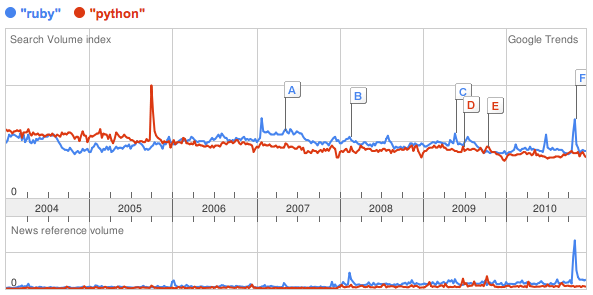
\includegraphics[width=0.8\textwidth,angle=0]{./bilder/ruby_vs_python.png}
        \caption{Google Trends, Vergleich Suchvolumen `Ruby' mit `Python'}
        \label{ruby_vs_python}
    \end{center}
\end{figure}

Wie man in der Grafik \ref{ruby_vs_python} sehen kann werden für beide Programmiersprachen
ungefähr gleich viele Suchabfragen durchgeführt.

\begin{figure}[ht]
    \begin{center}
        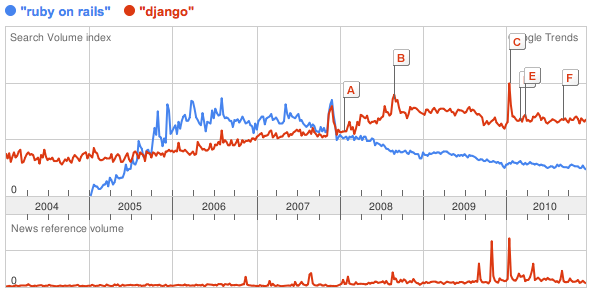
\includegraphics[width=0.8\textwidth,angle=0]{./bilder/ruby_on_rails_vs_django.png}
        \caption{Google Trends, Vergleich Suchvolumen `Ruby on Rails' mit `Django'}
        \label{ruby_on_rails_vs_django}
    \end{center}
\end{figure}

Vergleicht man die Frameworks `Ruby on Rails' und `Django' so kommt man laut ``Google Trends''
zu einem eindeutigen Ergebnis, was in der Grafik \ref{ruby_on_rails_vs_django} gut
zu erkennen ist.

Jedoch ist dies ein sehr treffendes Beispiel dafür, dass man ``Google Trends'' nicht auf
alles anwenden kann. Denn der Begriff `Django' wird nicht nur in Verwendung
mit dem `Python' Framework in Verbindung gebracht. Das sieht man, wenn man die Grafik
\ref{django_meldungen} betrachtet. Alle Nachrichten auf die ``Google Trends'' verweist,
haben überhaupt nichts mit dem Framework zu tun.

\begin{figure}[ht]
    \begin{center}
        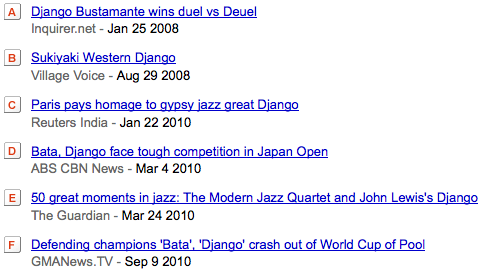
\includegraphics[width=0.8\textwidth,angle=0]{./bilder/django_meldungen.png}
        \caption{Google Trends, Nachrichten im Vergleich von `Ruby on Rails' mit `Django'}
        \label{django_meldungen}
    \end{center}
\end{figure}

Somit kann mich ``Google Trends'' bei der Entscheidung nicht unterstützen. Ich
entscheide mich für `Ruby on Rails', da ich darin mehr Erfahrung habe.

\clearpage

\subsection{Versionsverwaltungssystem}
Hier gibt es wiederum einige Systeme zur Auswahl \cite{versionsverwaltung}.
Jedoch schränke ich hier die Wahl auf Open-Source-Systeme ein und zwar auf
`Subversion', ein zentrales Versionsverwaltungs- und `Git', ein
verteiltes Versionsverwaltungssystem.

Ich habe mit beiden Versionsverwaltungssystem bereits gearbeitet und bin persönlich
mehr begeistert von `Git'. Ich habe damit schon viel gearbeitet und meine Projekte
auf der Plattform ``GitHub'' platziert. Diese Plattform ist sehr beliebt \cite{github}
und seit 2008 unteranderem dank `Ruby on Rails' bekannt geworden.

Wenn man `Subversion' und `Git' auf ``Google Trends'' vergleicht, sieht man auf
der Grafik \ref{svn_vs_git}, dass `Git' seit 2008 massiv an Suchanfragen zugenommen
hat.

\begin{figure}[ht]
    \begin{center}
        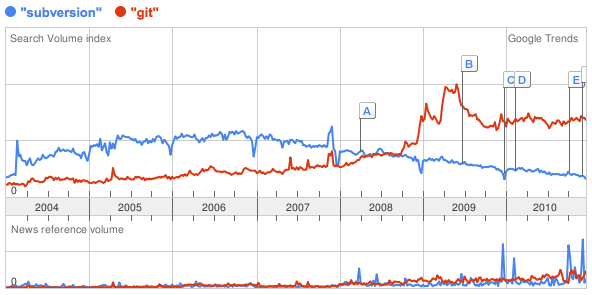
\includegraphics[width=0.8\textwidth,angle=0]{./bilder/svn_vs_git.png}
        \caption{Google Trends, Vergleich Suchvolumen `Subversion' mit `Git'}
        \label{svn_vs_git}
    \end{center}
\end{figure}

Ich entscheide mich deshalb für `Git' als Versionsverwaltungssystem und für ``GitHub''
als Hostingplattform für meinen öffentlichen Quellcode.

\section{Zusammenfassung}
Ich habe mich nach der Evaluation für eine Webapplikation, geschrieben mit `Ruby'
und unterstützt mit dem Framework `Ruby on Rails' entschieden. Als Versionsverwaltungssystem
habe ich `Git' gewählt und auf ``GitHub'' werde ich das Projekt inklusive dem Quellcode
veröffentlichen.